\section{RCIR+: its Type System and Semantics}
\label{sec:semantics}

As we have mentioned above, RCIR+ is a language for the purpose of compiling quantum oracle algorithms (or some other quantum algorithms, like Grover's algorithm, quantum walk and singular value transformation). Every quantum state in RCIR+ is represented by one of the three froms: $e^{\alpha}*|0>$ (or $e^{\alpha}*|1>$), $e^{\alpha}*(\pm|0>+\pm|1>)$, and $e^{\beta}*(|0> + e^{\alpha}*|1>)$. Based on the representation, we actually represent our quantum states as:

{
\[
rval = nat \to bool\qquad val = \texttt{nval}\; bool\;rval \;|\;\texttt{hval}\;bool\;bool\;rval\;|\;\texttt{qval}\;rval\;rval 
\]
}

Since all \texttt{Rz} gates in RCIR+ do rotations in the form either $2\pi i *\frac{1}{2^n}$ or $2\pi i *(1-\frac{1}{2^n})$, every angle rotation $\alpha$ in a state can be represented as a Boolean angle function $f$, whose meaning is defined as:

{
\[
 2\pi i * (\frac{1}{2^{1*(f(0))}} + \frac{1}{2^{2*(f(1))}} + ... + \frac{1}{2^{n*(f(n-1))}})
\]
}

\texttt{nval} is the state representation for $e^{\alpha}*|0>$ (or $e^{\alpha}*|1>$), and the Boolean value represents if the qubit state is $|0>$ or $|1>$. \texttt{hval} is the state representation for the form $e^{\alpha}*(\pm|0>+\pm|1>)$. The first Boolean value represents the $\pm$ sign for the $|0>$ qubit, and the second Boolean value represents the $\pm$ sign for the $|1>$ qubit. \texttt{qval} is to represent the states as the form $e^{\beta} * (|0> + e^{\alpha}*|1>)$. The first angle $rval$ represents $\beta$, while the second one represents $\alpha$ in the form with the semantic meaning described in the syntax above. In \texttt{Phi} mode, the only angle that can be rotated is $\alpha$.

For each state, we also have a type system to defines the type for it. The small type system has the following types:

\[
 type \;= \;\texttt{Nor}\; | \;\texttt{Had}\; |\; \texttt{Phi}\;nat
\]
 
The three different types refer to the three different modes of states described above. For a qubit state, it is impossible to have two kinds of states at the same time. \texttt{Nor} represents a state in \texttt{nval}, \texttt{Had} represents a state in \texttt{hval}, and \texttt{Phi} represents a state in \texttt{qval}. The natural number $nat$ associated with the \texttt{Phi} type represents the number of qubits that are related together in a QFT transformation. Turning a group of qubits to the \texttt{Phi} mode is essentially to do QFT on a group of qubits.  The type system will be associated with expressions in RCIR+. We first introduce the RCIR+ expressions here. Expressions in RCIR+ can be divided into three layers described in Fig.~\ref{fig:exp-layer}.

\begin{figure}[h]
\centering
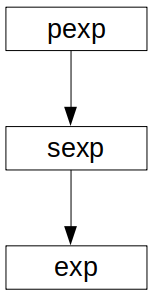
\includegraphics[width=0.15\textwidth]{exp_relation.png}
\caption{The Layer of Expressions in RCIR+}
\label{fig:exp-layer}
\end{figure}

The bottom level ($exp$) contains traditional quantum gates, like \texttt{X}, \texttt{CU}, \texttt{Rz} gates. On top of it, there is a set of operations ($sexp$) that deal with quantum state position swapping. Due to the virtual locations, the position swapping does not really have any effects in the actual physical quantum state locations. Instead, it changes the "view of qubits", which means we change the mapping from virtual state locations to physical locations. The top level ($pexp$) is to switch state space, which means that all operations there enforce certain type of state changes from one form to the other. We will discuss these expressions one by one. 

The syntax of the bottom level ($exp$) is described as follows:

\[
\begin{array}{l}
 exp \;= \texttt{SKIP}\; p \;|\; \texttt{X} \;p\; | \;\texttt{CU} \;p\; exp
        \;| \;\texttt{RZ} \;nat \;p
        \;|\; \texttt{RRZ} \;nat\; p 
\\\qquad
        \;|\; \texttt{SR}\; nat\; var
        \;|\; \texttt{SRR}\; nat\; var
        \;|\; \texttt{HCNOT} \;p\;p
        \;|\; \texttt{Seq} \;exp\; exp
\end{array}
\]

In $exp$, $p$ is a pair of a variable and a natural number. It represents the virtual location of a qubit state, and the application virtual location of a gate. The natural number ($n$, type: \texttt{nat}) appeared in the \texttt{RZ} and \texttt{RRZ} gates represents the rotation angle $2\pi i *\frac{1}{2^n}$ and $2\pi i *(1-\frac{1}{2^n})$, respectively. \texttt{RZ} represents actually the so-called \texttt{Rk} gate \cite{2000quant} in many traditional quantum gate descriptions, and \texttt{RRZ} is to apply an inverse \texttt{Rk} gate, which has the effect of applying the rotation $2\pi i *(1-\frac{1}{2^n})$ on the qubit state. 
\texttt{SR} gate is a special gate that is only used in \texttt{Phi} mode. It is actually a shortcut for a series of \texttt{RZ} gates. 
In \texttt{Phi} space, each qubit forms a suffix relation. In the first qubit in a \texttt{Phi} space, the $i$-th rotation position has to be the same as the $(i - m)$-th position for the $m$ qubit where $m\le i$. We call any of the rotation position across different qubits as linked rotation position. The \texttt{SR} gate is to enforce that every lined rotation position happened in \texttt{Phi} must rotate at the same angle every time. Otherwise, once we apply an inverted QFT after a rotation is applied to a \texttt{Phi} space, the system is not turned back to normal space. \texttt{SRR} is similar to \texttt{SR} but it contains a series of \texttt{RRZ} gates instead of \texttt{RZ} gates. \texttt{HCNOT} gate is essentially a \texttt{CNOT} gate with the restriction that the two positions must all in \texttt{Had} space. We will see examples of using these gates in the next section.

\begin{figure}[h]
\centering
\[\footnotesize
\begin{array}{l}
\begin{array}{llll}
\begin{array}{l}
\texttt{(1)}\;
\AxiomC{$$}
\UnaryInfC{$ \Gamma \vdash \texttt{SKIP}\;p$}
\DisplayProof
\end{array}
&
\begin{array}{l}
\texttt{(2)}\;
\AxiomC{$\Gamma(\texttt{fst}\;p)=\texttt{Nor}$}
\UnaryInfC{$ \Gamma \vdash \texttt{X}\;p$}
\DisplayProof
\end{array}
&
\begin{array}{l}
\texttt{(3)}\;
\AxiomC{$\Gamma(\texttt{fst}\;p)=\texttt{Had}$}
\UnaryInfC{$ \Gamma \vdash \texttt{X}\;p$}
\DisplayProof
\end{array}
&
\begin{array}{l}
\texttt{(4)}\;
\AxiomC{$\Gamma(\texttt{fst}\;p)=\texttt{Nor}\quad
 \Gamma\vdash e $}
\UnaryInfC{$ \Gamma \vdash \texttt{CU}\;p\;e$}
\DisplayProof
\end{array}
\end{array}
\\[2em]
\begin{array}{lll}
\begin{array}{l}
\texttt{(5)}\;
\AxiomC{$\Gamma(\texttt{fst}\;p_1)=\texttt{Had}\quad
 \Gamma(\texttt{fst}\;p_2)=\texttt{Had} $}
\UnaryInfC{$ \Gamma \vdash \texttt{CU}\;p_1\;p_2$}
\DisplayProof
\end{array}
&
\begin{array}{l}
\texttt{(6)}\;
\AxiomC{$\Gamma(\texttt{fst}\;p)=\texttt{Nor} $}
\UnaryInfC{$ \Gamma \vdash \texttt{RZ}\;q\;p$}
\DisplayProof
\end{array}
&
\begin{array}{l}
\texttt{(7)}\;
\AxiomC{$\Gamma(\texttt{fst}\;p)=\texttt{Had} $}
\UnaryInfC{$ \Gamma \vdash \texttt{RZ}\;1\;p$}
\DisplayProof
\end{array}
\end{array}
\\[2em]
\begin{array}{lll}
\begin{array}{l}
\texttt{(8)}\;
\AxiomC{$\Gamma(\texttt{fst}\;p)=\texttt{Nor} $}
\UnaryInfC{$ \Gamma \vdash \texttt{RRZ}\;q\;p$}
\DisplayProof
\end{array}
&
\begin{array}{l}
\texttt{(9)}\;
\AxiomC{$\Gamma(\texttt{fst}\;p)=\texttt{Had} $}
\UnaryInfC{$ \Gamma \vdash \texttt{RRZ}\;1\;p$}
\DisplayProof
\end{array}
&
\begin{array}{l}
\texttt{(10)}\;
\AxiomC{$\Gamma(x)=\texttt{Phi}\;n\quad
m<n $}
\UnaryInfC{$ \Gamma \vdash \texttt{SR}\;m\;x$}
\DisplayProof
\end{array}
\end{array}
\\[2em]
\begin{array}{ll}
\begin{array}{l}
\texttt{(11)}\;
\AxiomC{$\Gamma(x)=\texttt{Phi}\;n\quad
m<n $}
\UnaryInfC{$ \Gamma \vdash \texttt{SRR}\;m\;x$}
\DisplayProof
\end{array}
&
\begin{array}{l}
\texttt{(12)}\;
\AxiomC{$\Gamma \vdash \;e_1\quad \Gamma \vdash \;e_2 $}
\UnaryInfC{$ \Gamma \vdash \;\texttt{Seq}\;e_1\;e_2$}
\DisplayProof
\end{array}
\end{array}
\end{array}
\]
\caption{Well-Typed Definition For Exp}
\label{fig:exp-well-typed}
\end{figure}

The semantics of the expression is basically the same as ones appeared in SQIR. The only difference is that we are dealing with quantum states that are no entanglements. Therefore, the semantic description is more about to define the situation of applying different gates in the three modes of qubit states described above. The only tricky item here is that we have restrictions on the usage of different gates in different state modes. The relation that defines which gate is allowed to run on which mode is described in Fig.~\ref{fig:exp-well-typed}. In the figure, $\Gamma$ is a map from variables to modes. For example, \texttt{X} gates are allowed in the \texttt{Nor} and \texttt{Had} modes, while the control positions of \texttt{CU} gates are only allowed to run on the \texttt{Nor} mode, but the sub-expression of a \texttt{CU} gate can be run in other modes. \texttt{RZ} gate is fully allowed to run on the \texttt{Nor} mode, while if it is run on \texttt{Had}, the rotation angle is only allowed to be \texttt{1}, which means that the gate is a Pauli-Z gate. It is possible to extend the limitation to include \texttt{P} and \texttt{T} gates, but it will require more advanced state representation for \texttt{Had} mode. 
\texttt{SR} and \texttt{SRR} gates are \texttt{Phi} mode specific gates, while the two positions of \texttt{HCNOT} gates must be in the \texttt{Had} mode.

The second level expression ($sexp$) is mainly for swapping state positions. The syntax of $sexp$ is described as follows:

\[
sexp \;= \;\texttt{Lshift}\;x \;|\; \texttt{Rshift}\;x \;|\;\texttt{Rev}\;x 
                 \;|\; \texttt{Exp}\; exp \;|\; \texttt{SSeq} \;sexp\; sexp
\]

The variable $x$ in some expressions represents the virtual locations of a group of qubits. It has the same meaning as the first element of a pair $p$ appeared in $exp$. \texttt{Lshift} is to shift qubit virtual positions one step towards left for all qubits in $x$. If $x$ is allocated to have $n$ qubits, then, after the shift, the relation of the new state function $f'$ and the old one $f$ is: $f'(x,(i+1) \% n) = f(x,i)$ for $i=0,...,n-1$. \texttt{Rshift} is the opposite of \texttt{Lshift}, and the relation between $f'$ and old $f$ is: $f'(x,i) = f(x,(i+1)\%n)$ for $i=0,...,n-1$. \texttt{Rev} (the reverse operation) is to make the qubit positions up-side-down in $x$. Its semantic relation between $f'$ and old $f$ is given as: $f'(x,n-1-i) = f(x,i)$ for $i=0,...,n-1$.

The power of RCIR+ on dealing with these position swapping operations is that the compilations of these operations to SQIR all generate \textbf{zero} gates! During the compilation, instead of generating actually swap gates to do the operations, we actually change the mapping function from virtual qubit locations to its physical locations. For example, if we have a variable $x$ containing \texttt{4} qubits, and we applying a series of operations on it, such as $\texttt{SSeq}\;(\texttt{Lshift}\;x)\;e$. In this expression, $e$ is an expression that is applied to $x$ after the left-shift operation. Before applying the shift, let's assume that the compilation mapping is $\{(x,0) \mapsto 0, (x,1) \mapsto 1, (x,2) \mapsto 2, (x,3) \mapsto 3\}$. Then, after applying the shift, the compilation mapping becomes  $\{(x,3) \mapsto 0, (x,2) \mapsto 1, (x,1) \mapsto 2,(x,3) \mapsto 0\}$. Then, we also pass the mapping to deal with the applications in $e$. 

Since there is no \texttt{CU} gates in the $sexp$ and the top level, this mappings on each step can be generated during the program compilation time. One limitation is that, in RCIR+, one can never write a program with the \texttt{CU} gate on top of an expression containing these shift and reverse operations. We can call our shift/reverse operations as the static shift/reverse operations. If users really want the "dynamic" ones that live inside a \texttt{CU} gate, they can always define \texttt{SWAP} gates by using RCIR+. However, what we found out during the definition of the modulo-multiplication algorithm in RCIR+ is that we don't need to have "dynamic" shift/reserve operations and the static shift/reverse operations in RCIR+ can satisfy any needs in the algorithm. 

The top level expression ($pexp$) is to do another kind of "swapping" operations that swap/shift the qubit state modes, which is orthogonal with respect to the position swapping operations described above. The syntax of $pexp$ is described as follows:

\[
pexp \;=\; \texttt{SExp}\;sexp \;|\; \texttt{QFT} \;x \;| \;\texttt{RQFT}\; x
               \;|\; \texttt{H}\; x \;|\; \texttt{FSeq}\;pexp\;pexp
\]

\texttt{QFT} is to allow a quantum fourier transform (QFT) to all qubits in $x$, \texttt{RQFT} is the inverse QFT operation. \texttt{H} is a Hadamard gate. In the $sexp$ level, the types are actually not important since every shift/reverse operation can be applied in any mode. The types re-appear to be important in the $pexp$ level. The gates that live in this level actually shift the qubit state modes from one to the other. 

\begin{figure}[h]
\centering
\[\footnotesize
\begin{array}{l}
\begin{array}{ll}
\begin{array}{l}
\texttt{(13)}\;
\AxiomC{$\Gamma \vdash e$}
\UnaryInfC{$ (\Sigma,\Gamma) \vdash \texttt{SExp}\;e \triangleright \Gamma$}
\DisplayProof
\end{array}
&
\begin{array}{l}
\texttt{(14)}\;
\AxiomC{$\Gamma(x)=\texttt{Nor}\quad \Sigma(x)=n$}
\UnaryInfC{$ (\Sigma,\Gamma) \vdash \texttt{QFT}\;x\triangleright \Gamma[x\mapsto \texttt{Phi}\;n]$}
\DisplayProof
\end{array}
\end{array}
\\[2em]
\begin{array}{ll}
\begin{array}{l}
\texttt{(15)}\;
\AxiomC{$\Gamma(x)=\texttt{Phi}\;n$}
\UnaryInfC{$ (\Sigma,\Gamma) \vdash \texttt{RQFT}\;x\triangleright \Gamma[x\mapsto \texttt{Nor}]$}
\DisplayProof
\end{array}
&
\begin{array}{l}
\texttt{(16)}\;
\AxiomC{$\Gamma(x)=\texttt{Nor}\quad
 \Gamma\vdash e $}
\UnaryInfC{$ (\Sigma,\Gamma) \vdash \texttt{H}\;x\triangleright \Gamma[x\mapsto \texttt{Had}]$}
\DisplayProof
\end{array}
\end{array}
\\[2em]
\begin{array}{ll}
\begin{array}{l}
\texttt{(17)}\;
\AxiomC{$\Gamma(x)=\texttt{Had}$}
\UnaryInfC{$ (\Sigma,\Gamma) \vdash \texttt{H}\;x\triangleright \Gamma[x\mapsto \texttt{Nor}]$}
\DisplayProof
\end{array}
&
\begin{array}{l}
\texttt{(18)}\;
\AxiomC{$(\Sigma,\Gamma)\vdash e_1\triangleright \Gamma'
\quad(\Sigma,\Gamma')\vdash e_2\triangleright \Gamma'' $}
\UnaryInfC{$ (\Sigma,\Gamma) \vdash \texttt{FSeq}\;e_1\;e_2\triangleright \Gamma''$}
\DisplayProof
\end{array}
\end{array}
\end{array}
\]
\caption{Well-Typed Definition For PEXP}
\label{fig:pexp-well-typed}
\end{figure}

The well-typed definition for $pexp$ is listed in Fig.~\ref{fig:pexp-well-typed}. $\Sigma$ is an invariant map that records the number of qubits for each variable in the system. 
\texttt{QFT} can switch a state in the \texttt{Nor} mode to \texttt{Phi}, while \texttt{RQFT} can switch a state from \texttt{Phi} back to \texttt{Nor}. \texttt{H} gate switches the mode from \texttt{Nor} to \texttt{Had}, and switch a state in \texttt{Had} back to \texttt{Nor}.
The semantics of the $pexp$ gates has no essential difference from the same gates defined in SQIR. The only difference is that the gates are dealing with different qubit state representations than the ones in SQIR, and they also need to take care of mode switching.

\section{Example Quantum Circuits}
\label{sec:example}

In this section, we discuss the utility of RCIR+. As we mentioned above, we plan to utilize RCIR+ to analyze quantum circuits. The analysis means that doing property proofs, simulations, and random testing on quantum circuits. 
Here, we provide some example circuits that RCIR+ is capable of analyzing.

A trivial example of using RCIR+ is the ripple-carry adder \cite{ripple-carry}, since the gates used in the adder are essentially \texttt{X}, \texttt{CNOT}, and \texttt{CCX} gates, which are gates that can be analyzed in the \texttt{Nor} mode in RCIR+. 
A good example of using RCIR+ is probably the QFT-based arithmetic circuits. 

\begin{figure}[h]
\centering
     \begin{subfigure}[b]{0.6\textwidth}
         \centering
         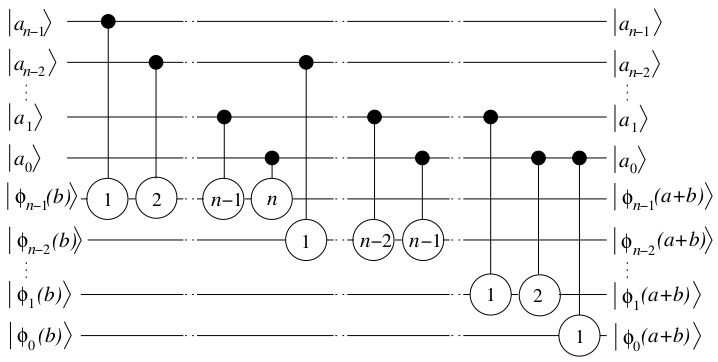
\includegraphics[width=1\textwidth]{qft-addition.png}
         \caption{QFT-based Addition Circuit}
         \label{fig:addition}
     \end{subfigure}%
     ~
     \begin{subfigure}[b]{0.6\textwidth}
         \centering
         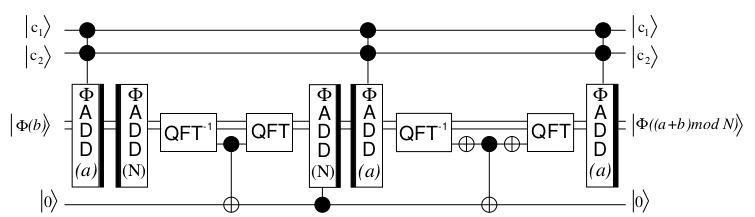
\includegraphics[width=1\textwidth]{qft-mod.png}
         \caption{QFT-based Modulo Multiplier Circuit}
         \label{fig:mod}
     \end{subfigure}

\caption{QFT-based Arithmetic Circuits}
\label{fig:qft-circuit}
\end{figure}

In Fig.~\ref{fig:qft-circuit}, we show the QFT-based addition circuit and a QFT-based modulo multiplier circuit. 
In Fig.~\ref{fig:addition}, the QFT-based addition circuit is assumed to have the input qubits for variable $b$ in the \texttt{Phi} mode, while qubits in variable $a$ are in the \texttt{Nor} mode.
To add the number $a$, which is represented as a binary Boolean values, to the $b$ value, it uses \texttt{CU} gates on variable $a$ qubits, and \texttt{RZ} gates for $b$. In RCIR+, we require gates in the \texttt{Phi} mode to only use \texttt{SR} and \texttt{SRR} gates. By exterminating the circuit carefully, we found that this is actually the case. For every qubit position $i$ in $a$, it touches only the $i$ rotation position in the rotation angle in each qubit of $b$. For example, the second $n-2$ qubit in $a$ rotates $\texttt{RZ}\;1$ in the $n-2$ qubit in $b$, and $\texttt{RZ}\;2$ in the $n-3$ qubit in $b$, and so on. We can conclude that an $n-i$ qubit in $a$ has \texttt{CU}-\texttt{RZ} gates on the $n-m$ qubit in $b$ where $m<i$, and the angle rotated in the $n-m$ qubit is $\texttt{RZ};(i-m+1)$. Hence, the \texttt{RZ} gates for each qubit in $a$ forms a \texttt{SR} gate in RCIR+. 
Fig.~\ref{fig:mod} show how to use mode transformation in RCIR+. We assume that the input for $b$ for the circuit is in the \texttt{Phi} mode, the two QFT-based addition circuits in the left can be done in the \texttt{Phi} mode, and the \texttt{RQFT} gate turns the mode of $b$ back to \texttt{Nor}, then it allows the \texttt{CNOT} gate (\texttt{CU} plus \texttt{X} gates) after \texttt{RQFT} is valid to run in the \texttt{Nor} mode. Then, the \texttt{QFT} gate turns $b$ back to \texttt{Phi}, and some other QFT-based addition operations can be applied on qubits in $b$. 

\begin{figure}[h]
\centering
         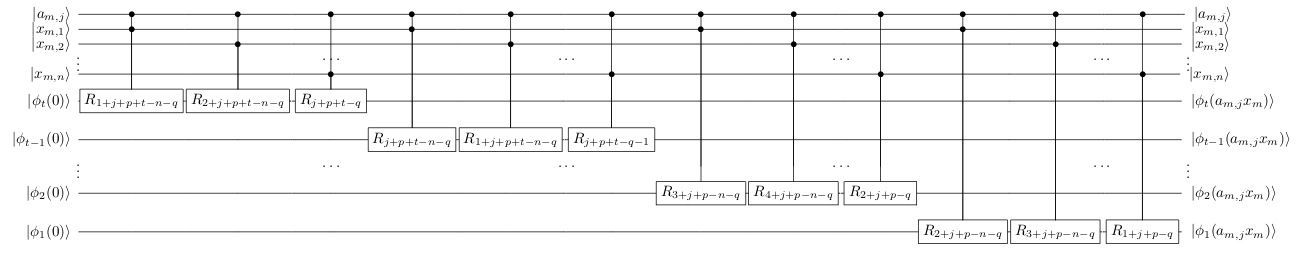
\includegraphics[width=\textwidth]{controlled-weight-sum.png}
\caption{QFT-based Controlled Weighted Sum Circuit}
\label{fig:qft-contol-circuit}
\end{figure}

Basically, all QFT-based arithmetic operations are analyzable by only using \texttt{SR} and \texttt{SRR} gates for \texttt{Phi}-mode qubits (obviously, we need other gates for qubits in the \texttt{Nor} mode). An example in the controlled weighted sum circuit in Fig.~\ref{fig:qft-contol-circuit}, which has the formula: $\Sigma^{2^n}_{m=1}a_m x_m$.

\begin{figure}[h]
\centering
     \begin{subfigure}[b]{0.6\textwidth}
         \centering
         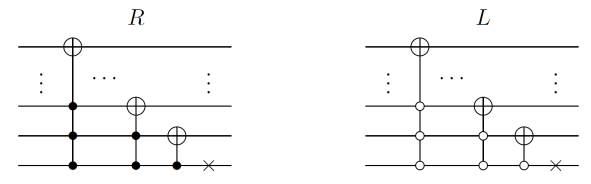
\includegraphics[width=1\textwidth]{lr-circuit.png}
         \caption{Circuits for L and R}
         \label{fig:lr-graph}
     \end{subfigure}

     \begin{subfigure}[b]{0.3\textwidth}
         \centering
         \includegraphics[width=1\textwidth]{circle-8-graph.png}
         \caption{Circle Graph (N = 8)}
         \label{fig:circle}
     \end{subfigure}%
     ~
     \begin{subfigure}[b]{0.7\textwidth}
         \centering
         \includegraphics[width=1\textwidth]{whole-quantum-walk.png}
         \caption{Full Circuit For Circle Graph Quantum Walk Oracle}
         \label{fig:quantum-walk-circle}
     \end{subfigure}

\caption{Quantum Walk Oracle Circuit}
\label{fig:circle-circuit}
\end{figure}

Another example circuit that can be analyzed is the oracle circuits in quantum walk in Fig.~\ref{fig:circle-circuit}. 
Most gates in the circuit are run in the \texttt{Nor} mode, and they can be analyzed by RCIR+. The only possible problem is the controlled-Z gate (\texttt{CZ}, listed as controlled $\pi$ in the Fig~\ref{fig:quantum-walk-circle}) surrounded by two \texttt{H} gates. In RCIR+, \texttt{CZ} gates are essentially \texttt{CU} gates and a $\texttt{RZ}$ gate with a rotation of angle $\pi$, and the \texttt{CU} gates are applied on qubits in \texttt{Nor}, as well as the \texttt{RZ} gate is applied on a qubit in the \texttt{Had} mode.
In Fig.~\ref{fig:quantum-walk-circle}, it seems that the \texttt{CZ} gate is applied on a controlled qubit in \texttt{Had} and all other qubits to be in \texttt{Nor}. What we find out is that these two \texttt{CZ} gate applications have the same effect. Any vector that is applied by a \texttt{CZ} gate where all controlled qubits are in \texttt{Nor} and the \texttt{RZ} applied qubit in the \texttt{Had} mode has the same effect as the one that is applied by a \texttt{CZ} gate where any one of the controlled qubit is in \texttt{Had} and all other qubits are in \texttt{Had}. This is why we are able to use RCIR+ to analyze the quantum walk oracle circuit in Fig.~\ref{fig:circle-circuit}.

\begin{figure}[h]
\centering
     \begin{subfigure}[h]{0.25\textwidth}
         \centering
         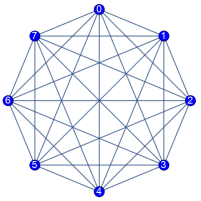
\includegraphics[width=1\textwidth]{k-graph.png}
     \end{subfigure}%
     ~
     \begin{subfigure}[h]{0.5\textwidth}
         \centering
         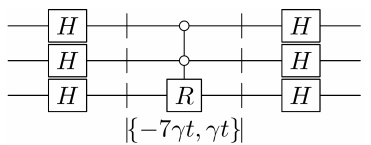
\includegraphics[width=1\textwidth]{tim-evolve-k-graph.png}
     \end{subfigure}
\caption{Quantum Walk Time-evolution Operator for $K_8$ Graph}
\label{fig:quantum-walk-time-evol}
\end{figure}

Unfortunately, not all quantum walk algorithm components are analyzable in RCIR+ with the qubit inputs to be in the \texttt{Nor} mode. 
Fig.~\ref{fig:quantum-walk-time-evol} shows a time-evolution operator in quantum walk for a $K_8$ graph.
This circuit is not analyzable in RCIR+ if the input qubits are in \texttt{Nor}.
To analyze this circuit in RCIR+, we first investigate an important theorem in dealing with quantum circuits in Observation~\ref{basic-state-thm}. 

\begin{observation}
\label{basic-state-thm}
\rm
If a quantum algorithm property is correct for all basis-vector inputs, the property can be extended for general quantum inputs.
\end{observation}

This Observation is a direct corollary from a theorem that is proved in the VOQC project \cite{10.1145/3434318}, where if two matrices produce the same output when they are multiplied by any basis-vector (a vector with $1$ in one row and $0$ in any other rows), then the two matrices are the same. An application of a quantum algorithm on an input is essentially to do a matrix multiplication on vectors as the input. The theorem tells us that if two algorithms are the same, then we only need to see if all basis-vectors as input for the two algorithms are the same. In contrast, if two quantum algorithms are tested to be the same under all basis-vectors, then we are not able to distinguish them by any input. In other word, if an algorithm property is correct in one algorithm $\sigma$, and there is another algorithm $\delta$ that is tested the same as $\sigma$ with all basis-vector inputs, then the property is also held in the algorithm $\delta$, because essentially algorithm properties are based on the input and output of algorithms. 

On the other hand, since all quantum algorithms are essentially matrix-vector multiplications, and any vectors can be viewed as a sum of scale multiplications of several basis vectors, if a property is held for all basis-vectors for an algorithm, the output behaviors of the property is calculable for arbitrary input vectors. 
This Observation can be extended to other forms of "basis" inputs for a quantum algorithms. Essentially, a basis-vector is a Kronecker product of qubits $|0>$ and $|1>$. One can produce a proportional relation between qubits $|+>$ ($\frac{1}{\sqrt{2}}(|0>+|1>)$) and $|->$ ($\frac{1}{\sqrt{2}}(|0>-|1>)$) are qubits $|0>$ and $|1>$. For example, $|0>\propto |+> + |->$. Hence, if a algorithm property is preserved for any Kronecker product of arbitrary $|+>$ and $|->$ (actually, we just need to analyze an arbitrary Kronecker product of exactly one $|->$ and many $|+>$), for arbitrary input qubits, the effects of the property is also calculable. 
For example, in dealing with the time-evolution operator in Fig.~\ref{fig:quantum-walk-time-evol}, if we assume that the input is an Kronecker product of $|+>$ and $|->$, then the inputs are in the \texttt{Had} mode, with the application of \texttt{H} gates, we can then analyze the effects of the \texttt{CU}-\texttt{RZ} gate in the middle. The quantum states to analyze in this format is a lot simpler than the ones if we assume that the input is with qubits $|0>$ and $|1>$. Additionally, if we keep the input as Kronecker products of $|+>$ and $|->$, in every computation step of the time-evolution operator, the quantum state is not entangled, which means that we can separately analyze every single qubit individually during the process. The direct consequence of analyzing the operator by using $|+>$ and $|->$ qubits is that we are able to design a traditional random testing algorithms to capture the behaviors for the time-evolution operator. We can then design the random testing kit in RCIR+ to have both inputs of Kronecker products of $|0>$ and $|1>$ (the \texttt{Nor} mode) and Kronecker products of $|+>$ and $|->$ (the \texttt{Had} mode) , so the random testing kit in RCIR+ now is able to show behaviors of more quantum algorithms. 

\begin{figure}[h]
\centering
         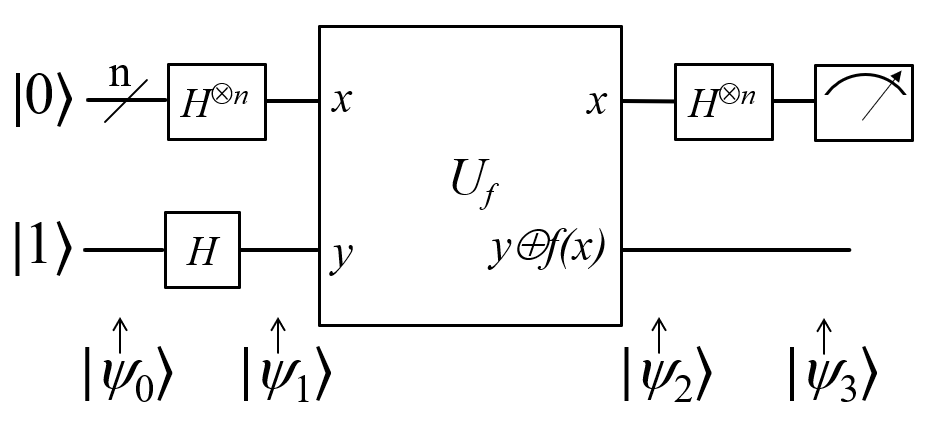
\includegraphics[width=0.5\textwidth]{deutsch-jozsa.png}
\caption{Deutsch-Jozsa Circuit}
\label{fig:Deutsch–Jozsa}
\end{figure}

A usage of the $|+>$/$|->$ qubit inputs is the analysis of the Deutsch–Jozsa algorithm (Fig.~\ref{fig:Deutsch–Jozsa}). By using the \texttt{Had} mode input, we are able to show the behaviors of step computations in this algorithm, and then for each step, we can produce the output behaviors of the algorithm with \texttt{Nor} mode input with a proper calculation. 

\section{An Example Usage of RCIR+: QSSA}
\label{sec:qssa}

One of the example usage of RCIR+ is the compilation of a high level SSA-formed (static single assignment formed) language with only arithmetic operations, such as math addition, subtraction, and multiplication, etc.

We first list the grammar of QSSA below:

\[
\begin{array}{l}
 fact \;= \texttt{Var}\; var \;|\; \texttt{Num} \;nat
\qquad
flag \;=\texttt{QFTA}\;|\;\texttt{Classic}
\qquad
bty\;=\texttt{Nat}\;|\;\texttt{Float}
\\[0.5em]
iexp \;=\texttt{plus}\;flag\;fact\;fact\;|\;\texttt{minus}\;flag\;fact\;fact\;|\;\texttt{mult}\;flag\;fact\;fact
\\\quad\;|\;\texttt{div}\;flag\;fact\;fact\;|\;\texttt{mod}\;flag\;fact\;fact\;|\;\texttt{load}\;var
\\[0.5em]
cexp \;=\texttt{clt}\;flag\;fact\;fact\;|\;\texttt{ceq}\;flag\;fact\;fact
\\[0.5em]
qexp\;=\texttt{inst}\;var\;nat\;bty\;iexp\;|\;\texttt{add}\;flag\;fact\;fact\;|\;\texttt{sub}\;flag\;fact\;fact
\\\quad\;|\;\texttt{times}\;flag\;fact\;fact
\;|\;\texttt{call}\;fvar
\;|\;\texttt{if}\;cexp\;qexp\;qexp
\;|\;\texttt{while}\;cexp\;qexp
\\\quad
\;|\;\texttt{ret}\;(list\;(var * var))
\;|\;\texttt{seq}\;qexp\;qexp
\\[0.5em]
fun\;=(fvar * qexp)
\qquad
prog\;=(nat * nat * nat * list\;(var * nat) * list\;fun)
\end{array}
\]

In QSSA, each variable is either a value representing a natural number (\texttt{Nat}) of a floating pointer number (\texttt{Float}). In addition, a variable can be either a global variable or a local variable. The expression \texttt{load} loads the value in a global variable to a local variable. The instruction \texttt{ret} returns a list of pairs of variables when a function is returned. In each pair $(x,u)$, $x$ must be a global variable and $u$ must be a local variable. The semantic meaning of \texttt{ret} for each pair $(x,u)$ is that $x:=u\oplus x$. From $iexp$, except \texttt{load}, all other expressions in QSSA are arithmetic operations. The $flag$ in each expression is either \texttt{QFTA} or \texttt{Classic}, meaning that the expression is computed using a QFT-based circuit and a classical circuit, respectively. $qexp$ represents instructions in a function. The basic instruction is $\texttt{inst}\;x\;n\;ty\;e$, where $x$ is the target variable to store the computation result, $n$ represents the number of bits in variable $x$, $ty$ defines if the value is a floating-point value or a natural number, and $e$ is an expression ($iexp$). All basic instructions $\texttt{inst}$ are required to be in SSA-format in a function, meaning that an variable $x$ in an \texttt{inst} can be assigned only once. For any \texttt{inst} having the form $x:=y\;\texttt{op}\;z$, it is corresponding to a reversible computation having the form as $[y][z][0]\rightarrow[y][z][x]$, where $x$ is the computation result of $y\;\texttt{op}\;z$.

In QSSA, we have a branching operation \texttt{if} and a loop operation \texttt{while}. Their Boolean guards are $cexp$ expressions. We currently allow users to compare if one value is smaller than the other one ($\texttt{clt}$), or if they are equal (\texttt{ceq}). 
In the body of a \texttt{while} loop in QSSA, we require that there is no basic instructions (\texttt{inst}). Instead, we provide three different operations for users in a loop body: \texttt{add}, \texttt{sub}, and \texttt{times}, with other kinds of instructions like \texttt{call}, \texttt{if}, \texttt{while}, \texttt{ret}, and \texttt{seq}. \texttt{add}, \texttt{sub}, and \texttt{times} represents math addition, subtraction, and multiplication, respectively. The difference between them and the ones in \texttt{inst} is the reversible computation formation. These three operations have the form: $[x][y]\rightarrow[x][y\;\texttt{op}\;x]$; so \texttt{add} can be better understood as "adding to", and \texttt{sub} is more like "subtracting from". We have the separation because of the efficiency concerns. Eventually, all variables in a QSSA function is mapped to an array of qubits. If we need to create a variable every time when a re-enter a loop body, this might not be feasible in the current status of a quantum circuit. Instead, most users might be interested in creating a variable before entering a loop, and updating the value in the variable when re-entering the loop. 
For each function ($fun$), there is also two global setting numbers that are related to the execution of a loop. The first number defines the stack size of a function, and the second number defines the maximum number of steps for executing a loop. The problem of having a loop in a quantum circuit is the loop Boolean guard. When executing a loop, every Boolean guard needs to be stored in a qubit, and for every step of computation, once a qubit is used for a Boolean guard, it cannot be re-used in the further step of loop-evaluation before the loop computation is finished. Hence, the compiler needs to know a place to swap clean ancillary qubits for storing a Boolean guard value.This is the so-called stack for a function, and the stack size for each function is pre-determined. In addition, for each loop execution, the maximum number of steps is also pre-determined, due to the fact that our compiler needs to expand the loop code before executing the loop operation.

In QSSA, function calls have no arguments at this point, and it is also not recursive. The usage of a function is to provide a automatic inverse circuit. For a function having the form: $f()\{e;\texttt{ret}\; l\}$, it is actually to execute the following: $e;\texttt{ret}\; l;\texttt{inv}\;e$. We first evaluate the function body $e$, and then the return instruction copies all local variables to global variables, and then we do an inverse of the function body $e$ (\texttt{inv}). 

Now, we discuss some about the compilation and type system of QSSA. Each variable in QSSA is having a type that is represented as a tuple of two different type fragments as: 

\[
\begin{array}{l}
bty\;=\texttt{Nat}\;|\;\texttt{Float}
\quad
aty\;=\texttt{C}\;nat\;|\;\texttt{Q}\;nat
\quad
type\;=(aty * bty)
\\[0.5em]
\end{array}
\]

Other than the \texttt{bty} fragment to classify if a variable representing a float or a natural number, the \texttt{aty} fragment checks if the value of a variable is "statically" determinable or "dynamically" determinable. 
The meaning of "statical"/"dynamical" determination is different from the version used in a classical compiler field. Here, we refer to statically determinable variable as its value is commutable without using quantum circuits, while dynamically determinable variable must hand to a quantum circuit to compute its value. The logic behinds this classification is that any effective computation that is compatible in a classical computer is a lot "cheaper" than doing the computation in a quantum machine.
The QSSA type system and compiler aggressively checks every line of code in a function and finds statically determinable variables as much as possible and per-compute all values for all statically determinable variables, and then we generate quantum circuits for only dynamical determinable variables.

A key observation of doing the compilation from QSSA to RCIR+ is that every operation in QSSA is a computation starting at a \texttt{Nor} mode and also ends at a \texttt{Nor} mode. If we think of the instruction in QSSA in terms of a compiled circuit in RCIR+, we find that the input for every operation is basically a series of qubits $|0>$ and $|1>$, and the output for every operation is also a series of $|0>$ and $|1>$. No matter the middle circuit is a QFT-based or a classical circuit, if the starting mode is \texttt{Nor}, then the ending mode is also \texttt{Nor}. This observation ease the compilation proofs from QSSA to RCIR+, and it also enables us to have a rich language representation.

One final thing worth noting is that QSSA is an example of using RCIR+. RCIR+ might enables more operations than the set of QSSA instructions listed here, such as the graph oracles and time evolving operators in quantum walk algorithms. For some enhanced quantum oracles or algorithm components, users might want to write their own effective circuit implementation in RCIR+. The RCIR+ random testing kit provides a way for helping users to validate and debug their large circuit implementations without going through the "pain" of proving the correctness of a compiler. 

\section{Evaluation and Future Study}
\label{sec:eval}
 
Currently, I have finished implementing the type system and semantics for RCIR+. I have already proved the correctness of compilation from RCIR+ to SQIR for $exp$ and $sexp$. I also the classical and QFT-based modulo multiplier on RCIR+, as well as the correctness proof for the classical modulo multiplier. There are several takeaways here. 

First, RCIR+ solves the problem of "can". By using RCIR+, we are able to define the classical and QFT-based adders and other oracle algorithms in a \textbf{single} framework. I also plan to define Grover's algorithm, as well as quantum walk algorithms in RCIR+. 
Second, RCIR+ also helps reduce the compilation gates. In dealing with the classical modulo multiplier, we are able to reduce 60\% of the
gates when we compile the circuit to SQIR. This is mainly because the fact that we don't need to do any static shift/reverse operations as well as reduce many swap operations. 
Third, RCIR+ helps the problem of "simplification". In defining the modes and restricting when a gate can be applied, we are able to avoid qubits having entanglements. This will certainly help simplifying the analysis of many quantum algorithms, especially oracle algorithm, that do not rely on entanglements. 
In addition, we can simplify the design of an RCIR+ simulator because the three different modes of qubit states that are based on natural numbers can improve the performance. 

For future study, I plan to define the sine/cosine functions based on the cordic method that relies on addition and shift operations, as well as many quantum oracles and components in quantum walk. Since I have finished the design for classical and QFT-based modulo multipliers, these automatically give us the addition, subtraction, and multiplication operations. These can be the basis of the compilation from QSSA to RCIR+. I can imagine the compilation will be easy to do since we have all separated components. Please feel free to talk to me and I need cooperation. 



